% Document class options:
% =======================
%
% lineno: Adds line numbers.
%
% serif: Sets the body font to be serif. 
%
% twocolumn: Sets the body text in two-column layout. 
% 
%
% Using other bibliography styles:
% =======================
% Not supported at the moment
\documentclass[twocolumn, serif, authordate, review]{jote-article}


%%% Add the bibliography, make sure it's in the same directory
%\addbibresource{traxler.bib}

%%% Add additional packages here if required. Usually not needed, except when doing things with figures and tables, god help you then

% This package is for generating Lorem Ipsum, usage: \lipsum[X] where X is the Xth paragraph of lorem ipsum. OR use [1-5] to generate the first five, etc.
\usepackage{lipsum}


% Fill in the type of article here. Doesn't matter if capitalized. 
%%% Options
% Empirical
% Reflection
% Meta-Research
% Rejected Grant Application
% Editorial
%%% TODO: Make this a 1-5 option scale to reduce the chance of mistyping
\papertype{Empirical}

% Enter the title, in Title Case Please
% Try to keep it under 3 lines
\title{Trial and Error (-Related Negativity): An Odyssey of Integrating Different Experimental Paradigms}

% List abbreviations here, if any. Please note that it is preferred that abbreviations be defined at the first instance they appear in the text, rather than creating an abbreviations list.
%\abbrevs{ABC, a black cat; DEF, doesn't ever fret; GHI, goes home immediately.}

% Include full author names and degrees, when required by the journal.
% Use the \authfn to add symbols for additional footnotes and present addresses, if any. Usually start with 1 for notes about author contributions; then continuing with 2 etc if any author has a different present address.

\author[1]{Ilona Domen}
\author[2]{Kristel De Groot}

\ogauthor{Juliane Traxler, Roxane V. Philips, Andreas von Leupoldt, Johan W. S. Vlaeyen}
%Fill it in again for the PDF metadata. Lame workaround but it works

%List the contribution effort here, they will be listed at the end of the page
%\contributions{Equally contributing authors.}

% Include full affiliation details for all authors
\affil[1]{Reviewer 1}
\affil[2]{Reviewer 2}

% Optionally list the present address of one of the authors
%\presentadd[\authfn{2}]{Department, Institution, City, State or Province, Postal Code, Country}

% Fill in the DOI of the paper

% Always starts with "10.36850/" and is suffixed with one of the following plus a number
% e  : empirical
% r  : reflection
% mr : meta-research
% rga: rejected grant application
% ed : editorial
\paperdoi{10.36850/e2}

% Include the name of the author that should appear in the running header
\runningauthor{Traxler et al.}

% The name of the Journal
\jname{Journal of Trial and Error}

% The year that the article is published
\jyear{2020}

%The Volume Number


%The website that's listed in the bottom right
\jwebsite{https://www.jtrialerror.com}

%%% Only \paperpublished is necessary, any combination of the other two is possible

%When the paper was received

% When the paper will be published
\paperpublished{16 December, 2020}
% When the paper is published but in YYYY-MM-DD format, for the crossmark button
\paperpublisheddate{2020-12-16}

% The pages of the article, comment out if rolling article
%\jpages{1-12}
% Link to the logo, might be redundant
\jlogo{media/jote_logo_full.png}

% Fill something here if this is a rolling/online first article, will make ROLLING ARTICLE show up on the first page
%\rolling{YES}

% Sets the paragraph skip to be zero, this should be in the CLS
\setlength{\parskip}{0pt}

%%% Companion Piece

% Reflection and Empirical articles have each other as companion pieces. Add the DOI, Title, and Abstract of the respective Companion piece here
\companionurl{https://doi.org/10.36850/r2}
\companiontitle{Derksen (2020)}
\companionabstract{`Trial and Error (-related negativity)' is a fascinating paper detailing the attempt to develop a new experimental paradigm to study the role of error-related negativity in the development of avoidance behavior. In my comments on this paper I will focus on the interaction between experimenters and participants as the former investigate various ways of designing the experiment, aiming to elicit the right kind of behavior from the participants. As in many psychological experiments, there is a fundamental tension here that experimenters must find a way to deal with: they must guide the subject to the proper performance, without the subject responding to the guidance as such. The performance must be natural, but within tight constraints. Recalcitrance or resistance of the subject must be prevented. Ultimately, the authors of ‘Trial and Error (-related negativity)’ failed in their attempt to do this. Their reflections on their failure are thorough and illuminating, but I will argue that they can be pushed slightly further.}
\companionkey{Derksen2020}
%%% Abstract

% These two set the height and width of the abstract. There's no solution to do this automatically at the moment so fiddle with these a bit. height-width should be 5mm, and ranges between 50-100 are realistic
% Higher number means skinnier abstract
\heightabstract{48mm}
\widthaffil{43mm}
%Enter something here in order for the abstract to disappear. Be sure to also delete the abstract 
\noabstract{}
% Fill in the keywords that will appear in the abstract, max 7
\keywordsabstract{error-related negativity, avoidance behavior, chronic pain, experimental psychopathology, experimental paradigm}

%%%%%%%%%%%%%%%%%%%%%%%%%%%%%%%%%%%%%%%%%%%%%%%%%%%
%Document Starts
%%%%%%%%%%%%%%%%%%%%%%%%%%%%%%%%%%%%%%%%%%%%%%%%%%%

\begin{document}
%%% This starts the frontmatter, which includes everything that's on the front page execpt the text of the article
\begin{frontmatter}
\maketitle
%Type your abstract between these things. Max 250 words. Be sure to include the \noindent, looks bad otherwise
\begin{abstract}
Pain can be considered as a signal of ``bodily error'': Errors -- discrepancies between actual and optimal/targeted state -- can put organisms at danger and activate behavioral defensive systems. If the error relates to the body, pain is the warning signal that motivates protective action such as avoidance behavior to safeguard our body's integrity. Hence, pain shares the functionality of errors. On the neural level, an important error processing component is the error-related negativity (ERN), a negative deflection in the electroencephalographic (EEG) signal generated primarily in the anterior cingulate cortex within 100 ms after error commission. Despite compelling evidence that the ERN plays an important role in the development of various psychopathologies and is implicated in learning and adjustment of behavior, its relation to pain-related avoidance has not yet been examined. Based on findings from anxiety research, it seems conceivable that individuals with elevated ERN amplitudes are more prone to engage in pain-related avoidance behavior, which may, under certain conditions, be a risk factor for developing chronic pain. Consequently, this new line of research promises to contribute to our understanding of human pain.

As in most novel research areas, a first crucial step for integrating the scientific fields of ERN and pain is developing a paradigm suited to address the needs from both fields. The present manuscript presents the development and piloting of an experimental task measuring both ERN and avoidance behavior in response to painful mistakes, as well as the challenges encountered herein. A total of 12 participants underwent one of six different task versions. We describe in detail each of these versions, including their results, shortcomings, our solutions, and subsequent steps. Finally, we provide some advice for researchers aiming at developing novel paradigms.

Take-home message: Developing a new experimental paradigm is challenging, time-consuming and requires thorough testing. To make this process most efficient, we advise to clearly define the requirements at the beginning, to keep record of all decisions and adjustments made in the process, and to investigate encountered problems and failures which may help to gradually improve the paradigm.

\end{abstract}
\end{frontmatter}

%% Purpose




\phantomsection 
\addcontentsline{toc}{section}{Purpose}
\section*{Purpose} 
\gotoreview
\label{sec:purpose}

\noindent Avoidance behavior is part of a natural defense mechanism that is activated when individuals are experiencing chronic pain. In order to shed more light on the neural underpinnings of pain avoidance behavior, it is our long-term aim to investigate its association with the error-related negativity (ERN), an important component of neural error processing. So far, the ERN has been predominantly examined in relation to anxiety disorders, and has been suggested as an endophenotype of obsessive-compulsive disorder (Riesel et al., 2011). Initially, ERN research focused on its relationship with the tendency to learn best from negative feedback (Frank et al., 2005), whereas a few more recent studies also observed greater disorder-specific defensive motivation and avoidance behavior in individuals with elevated ERN amplitudes (Riesel, 2019; Riesel et al., 2019; Weinberg et al., 2016). These findings support the assumption that the ERN may be similarly implicated in pain-related avoidance but this possibility remains to be tested.~Investigating this theoretically plausible association may generally improve our understanding of the neural mechanisms underlying avoidance behavior and help to identify individuals at risk of developing chronic pain.~The novelty of this endeavor requires the integration of knowledge of both research strands, as well as the development of an experimental paradigm that is suited to meet their respective requirements. Here, we describe the process of developing and piloting such a paradigm, and provide an overview of problems encountered herein. We conclude with a tutorial section on the development of novel experimental paradigms based on our experience with this specific study, which we hope is also broadly applicable.


\phantomsection 
\addcontentsline{toc}{section}{Introduction}
\section*{Introduction} 
\gotoreview
\label{sec:introduction}

\noindent Chronic pain affects as many as 20\% of adults in Europe (Societal Impact of Pain, 2017). This poses a considerable health care challenge and tremendous individual suffering. One of the most prevalent explanations for the transition from a common acute pain episode to chronic disabling pain is the fear-avoidance model (Vlaeyen et al., 2016; Vlaeyen \& Linton, 2000; Vlaeyen \& Crombez, 2020). It posits that pain-related avoidance behavior, often fueled by catastrophic (mis)interpretations of pain, contributes to individuals entering into a downward spiral of fear, avoidance, inactivity, disability and negative affect. Pain-avoidance refers to individuals avoiding stimuli that are predictive of pain or pain exacerbations. For instance, persons who have sustained an injury to their back, may avoid lifting objects for fear that it will lead to further pain, or fear that lifting may create bodily harm that is signaled by pain. Typically, avoidance occurs in anticipation of pain, and hence individuals have little opportunity to test and, if necessary, correct their beliefs about the threat associated with such activities. This failure to correct mistaken beliefs maintains pain-related fear and further increases mood disturbances and pain itself (van Vliet et al., 2018; Vlaeyen \& Linton, 2000).~

The neural underpinnings of pain-related avoidance behavior are poorly understood. A new and promising avenue to understanding pain-related avoidance is to study its relation to error-related negativity (ERN). The ERN is an event-related potential (ERP), which occurs within $\mathrm{\sim}$100ms after error commission (Hajcak, 2012). It can be measured as a negative deflection in the electroencephalogram (EEG) over fronto-central scalp positions, originating in the anterior cingulate cortex (Miltner et al., 2003). Differences in the amplitude of the ERN are affected by both contextual and individual factors such as motivational aspects and error salience, and are considered to reflect individual error sensitivity (Hajcak, 2012; Hajcak \& Foti, 2008). For instance, it has been observed that the ERN is larger when errors are perceived to have worse consequences (Hajcak, 2012). Additionally, the ERN is believed to activate a defensive motivational system, in order to adjust the erroneous behavior and protect the organism (Hajcak \& Foti, 2008). In line with these findings, increased ERN amplitudes have consistently been associated with anxiety disorders (Weinberg, Riesel \& Hajcak, 2012) as persons affected arguably perceive their own mistakes in relation to the respective object of fear as highly threatening.~In addition, avoidance behavior (including experiential avoidance) is a typical feature of anxiety disorders (Aupperle \& Martin, 2010; Berman et al., 2010; Dikman \& Allen, 2000; Dymond \& Roche, 2009).

Given the commonalities between anxiety disorders and chronic pain (Asmundson \& Katz, 2009), and the high prevalence of negative affect in chronic pain (Geisser et al., 2000), it is theoretically plausible that the ERN may be a biomarker for the development of pain-related avoidance behavior as well. In the case of anxiety the particular fear object is considered threatening, whereas individuals with chronic pain perceive pain to be highly threatening. Due to pain being such a salient and aversive stimulus, as well as conceptually signaling bodily error, avoidance responses constitute a defensive mechanism to prevent the feared outcome (Leeuw et al., 2007). As such we may see an association between the ERN amplitude and the level of avoidance exhibited by an individual, with avoidance representing a defensive behavior in response to a motivationally salient and aversive stimulus.~

Our long-term goal is to investigate whether individual differences in the ERN amplitude are related to differences in pain-related avoidance behavior, which may help identify individuals more at risk for the development of chronic disabling pain. To this end, we aimed at creating an experimental paradigm that would allow us to measure the ERN and avoidance responses simultaneously, the process of which is described in the present manuscript. A task integrating both the ERN and avoidance is more efficient than measuring them in separate tasks. It ensures that there is a relation between error commissions and pain-related avoidance and puts less burden on the participant. Such a paradigm would need\textbf{ }to meet requirements for both measures, ERN and pain-related avoidance, namely: 1. evoke an ERN; 2. yield a reliable estimate of the ERN, requiring a minimum of six errors (Olvet \& Hajcak, 2009); and 3. be able to detect individual differences in avoidance behavior by providing sufficient opportunities to avoid (at least 20). Although there is some debate as to whether one needs to be aware of having committed an error to evoke the ERN (Nieuwenhuis et al., 2001), awareness is essential in this task as participants would otherwise be unable to perform the avoidance response. In addition, the task ought to evoke inhibition errors rather than mistakes due to lack of skill or knowledge. For that purpose, we decided to integrate two experimental tasks, one of which is frequently used to measure the ERN [the Eriksen Flanker task (Eriksen \& Eriksen, 1974)] and the other is a common assessment of avoidance behavior [the avoidance task by Vervliet and Indekeu (2015)]. We piloted this basic paradigm and continuously adjusted it based on the pilot results, leading to a total of six task variations. The focus of the present article is the design and execution of these different tasks, what we can learn from them and suggestions for future research.~


\phantomsection 
\addcontentsline{toc}{section}{Methods}
\section*{Methods}  
\gotoreview
\label{sec:methods}

\phantomsection 
\addcontentsline{toc}{subsection}{Participants} \subsection*{Participants}
\gotoreview
\label{sec:participants}

\noindent Twelve participants (8 females) took part in the pilot study between January and March of 2020. They were recruited by word of mouth, had a mean age of M = 29.25 (SD = 10.64), and gave autonomous consent. The exclusion criteria were self-reported: (a) pregnancy, (b) diagnosis of a psychiatric disorder (e.g. depression, anxiety, etc.), (c) a serious medical illness (e.g. diabetes mellitus, cardiovascular disease, neurological problems, etc.), (d) skin disease or condition where electrocutaneous stimuli could cause damage (e.g. an operation scar at the site where the electrodes would be placed), (e) pain: acute (e.g. due to an injury) or chronic, (f) electronic implant (e.g. pacemaker), (g) having been asked by a doctor to avoid stressful situations, and (h) poor vision or hearing that is not corrected. Pilots provided written informed consent at the onset of the experimental session. The procedures conformed to the Helsinki Declaration and were approved by the institutional ethics committee (Social and Societal Ethics Committee; approval reference number: G-2019 12 1905).~

\phantomsection 
\addcontentsline{toc}{subsection}{Apparatus}
\subsection*{Apparatus}  

\phantomsection\addcontentsline{toc}{subsubsection}{Electroencephalography}\subsubsection*{Electroencephalography}Event-related potentials in response to errors and correct trials were measured by means of electroencephalography (EEG) which was continuously recorded from the scalp using a 129-channel system (HydroCel Geodesic Sensor Net, Philips Electrical Geodesics Inc., Eugene, USA). The sampling rate was set at 250 Hz, electrode impedances were kept below 50 k? and the vertex electrode was used as reference point.

\phantomsection\addcontentsline{toc}{subsubsection}{Stimulation}\subsubsection*{Stimulation}Vibrotactile stimuli were administered to the left side of participants' lower back through two vibrotactors (Dancer Design, St Helens, England) placed 2 cm apart (center to center; Figure 1). The stimulus duration was 112 ms and the vibration intensity, which was set to a clearly perceptible level that remained non-painful throughout the experiment, was kept constant across participants. Tactors were activated in a semi-randomized order.

Electrocutaneous stimuli (e-stim) were generated by a constant-current stimulator (DS7A; Digitimer, Welwyn Garden City, England) and delivered for a duration of 2 ms through two 4mm Ag/AgCl reusable snap electrodes filled with K-Y gel attached 1 cm above the vibrotactors. The intensity of these stimuli was individually calibrated to a level that was ``painful and demanding some effort to tolerate''. For that purpose, a series of stimuli of ascending intensity was administered, each of which participants were instructed to verbally rate on a scale ranging from 0 (no sensation) to 10 (worst imaginable pain). The calibrated stimulus intensity was kept constant throughout the task.

The lower back was selected as stimulus location for two reasons: 1. the sensory acuity at the back is relatively low compared to more typical distal stimulation sites, such as the arms or hands (Weissman-Fogel et al., 2012), which was considered advantageous with regard to task difficulty; and 2. a large, even surface area was required to attach the vibrotactors and electrodes.

\phantomsection\addcontentsline{toc}{subsubsection}{Software}\subsubsection*{Software}The experimental task was programmed and presented in Affect 5 (Spruyt et al., 2009), which was run on a Windows 7 Professional (Microsoft Corporation Redmond) 64 bit Dell OptiPlex 780 (Dell Inc, Round Rock, TX) with 4-GB RAM, Duo-CPU at 3.10 GHz.


\phantomsection\addcontentsline{toc}{subsubsection}{Measures}\subsubsection*{Measures}

The purpose of the pilot study was to create a task that allows to measure the ERN and avoidance behavior simultaneously. In each task version vibrotactors emitted vibrations on participants' left lower back, EEG in response to correct and error trials was recorded, and painful e-stim were applied when participants made an erroneous response which they could omit by pressing the space bar. Avoidance was operationalized as the number of button presses to cancel an e-stim.

After performing the task participants were asked questions to receive their perspective of the task and to ensure that requirements were met. Specifically, they were asked whether they were able to perceive when they made errors, how difficult they found the task as well as initiating the avoidance response, and any additional comments they would like to provide.

\phantomsection 
\addcontentsline{toc}{subsection}{General procedure}
\subsection*{General procedure} 
\gotoreview
\label{sec:procedure}

\noindent All task versions were based on a tactile task that was inspired by Eriksen's Flanker task (Eriksen \& Eriksen, 1974) and a fear-avoidance paradigm established by Vervliet and Indekeu (2015). In the tactile task participants were instructed to distinguish between locations of vibrations emitted on their left lower back. Much like the arrow version of the Eriksen Flanker task, in which the direction of arrows is the cue for a correct response, participants used left and right mouse buttons to indicate whether they felt a vibration at the left or right location, respectively. Participants were instructed to respond as quickly and as accurate as possible. In addition, participants were informed that upon error commission they would receive an electrocutaneous stimulus, which they could cancel by pressing the space bar on the keyboard. Tasks employed either two or three vibrotactors (Figure 1).~


\begin{figure}
    \centering
    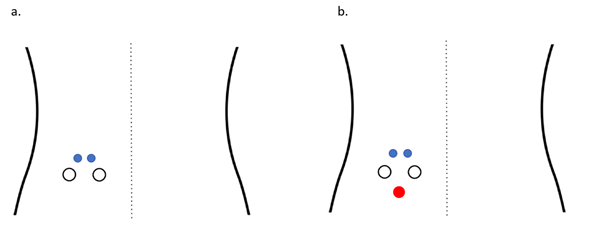
\includegraphics[width=\columnwidth]{articles/empirical/traxler/Figure 1_Trial and Error (-Related Negativity) (5).png}
    \caption{Electrode and tactor placements, with electrodes in blue. (a) Two tactor placement. (b) Three tactor placement with the red tactor indicating the distractor tactor.}
    \label{fig:1}
\end{figure}

A typical trial proceeded as follows (see Figure 2): a vibration was emitted (112ms), followed by a response window, to indicate the location of the vibration (200-1000ms). After a fixation period (300ms), participants could provide an avoidance response (1000ms). If participants chose not to avoid the e-stim upon error commissioning, an e-stim was delivered following this response window. The trial concluded in a jittered intertrial interval (600-1000ms). To prevent `better safe than sorry' reasoning for performing the avoidance response, participants were told that five, and later two, trials would be added to the duration of the experiment every time they cancelled an e-stim. In reality, no trials were added. As this proved to be highly aversive to the participants, leading to an unwillingness to avoid, we removed this clause after the eighth participant. Any deviations from the general procedure will be indicated.~Table 1 indicates the total number of participants and trials per task version. In general, the task versions were composed of four or five blocks of 60 trials each. In total, six different versions of the task were tested: \textit{Two Tactor task}, \textit{Distractor task}, \textit{100\% coactivation task}, \textit{Different intensities task}, \textit{50\% coactivation task}, and a \textit{Sequence task}.

\begin{figure}
    \centering
    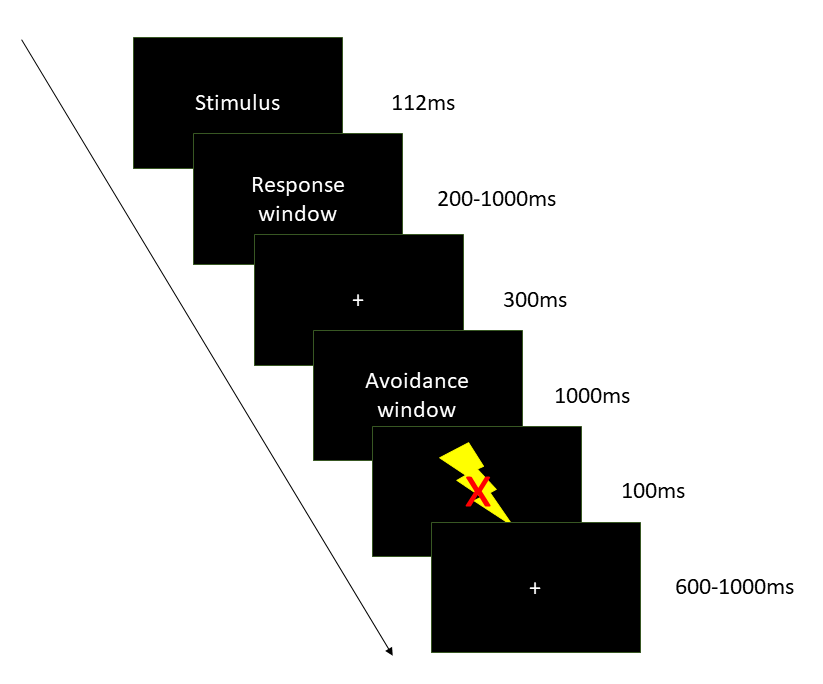
\includegraphics[width=\columnwidth]{articles/empirical/traxler/Figure 2_Trial and Error (-Related Negativity) (5).png}
    \caption{Schematic representation of the basic trial flow with exact timings depending on the task version.}
    \label{fig:my_label}
\end{figure}


\begin{table*}\sffamily
\begin{tabularx}{\textwidth}{@{}p{0.17\textwidth}p{0.12\textwidth}p{0.17\textwidth}p{0.12\textwidth}X}
\toprule Task & Number of Tactors & Stimulation intensity & Number of tasks & When does the distractor tactor activate?\tabularnewline \midrule 
Two Tactor & 2 & equal & 1 & NA\tabularnewline Distractor & 3 & equal & 2 & Plays a song\tabularnewline 100\% coactivation & 3 & equal & 1 & With every target stimulus\tabularnewline Different Intensities & 3 & 3rd tactor more intense & 1 & With every target stimulus\tabularnewline 50\% Coactivation & 3 & equal & 1 & With 50\% of target stimuli\tabularnewline Sequence & 3 & equal & 1 & With every target stimulus\tabularnewline \bottomrule 
\end{tabularx}
\caption{Overview of manipulations over task versions.}
\label{tab:manipulations}
\end{table*}

\emph{Note.} Number of tasks refers to whether participants had to perform any additional tasks to the discrimination task. \emph{Tasks are listed in the order in which they were tested.}

\phantomsection 
\addcontentsline{toc}{subsection}{Two Tactor task}
\subsection*{Two Tactor task}
\gotoreview
\label{sec:twotactor}
\phantomsection\addcontentsline{toc}{subsubsection}{Procedure}\subsubsection*{Procedure}In this first version of the task, two tactors were attached to the left lower back of the participants (Figure 1, a). Participants indicated via left and right mouse button press whether they felt a vibration at the left or right location, respectively. Upon error commission participants were free to cancel the e-stim by pressing the space bar.~One participant completed four blocks of this task version.

\phantomsection\addcontentsline{toc}{subsubsection}{Evaluation}\subsubsection*{Evaluation} After running one participant it was quickly established that this task was too easy. This was reflected by participant feedback, as well as the number of errors (\textit{M${}_{error\ }$}= 2).~The participant was aware of having made mistakes, but chose not to give any avoidance responses.

\phantomsection 
\addcontentsline{toc}{subsection}{Distractor task}
\subsection*{Distractor task}
\gotoreview
\label{sec:distractor}
\phantomsection\addcontentsline{toc}{subsubsection}{Procedure}\subsubsection*{Procedure}In order to increase task difficulty,\textbf{ }three tactors were attached to the left lower back, with two at the original locations and the third centrally below them (Figure 1, b).\textbf{ }This distractor tactor was emitting vibrations to the beat of a widely known song (e.g., ``Seven Nation Army'' by The White Stripes). The participant was instructed to respond exclusively to left and right vibrations. At the end of each block they had to choose, in a multiple choice manner, which song the third tactor had been vibrating to.~One participant completed four blocks of 60 trials.~

\phantomsection\addcontentsline{toc}{subsubsection}{Evaluation}\subsubsection*{Evaluation}There were several issues with this task version. The task appeared to be difficult, which led to the participant being exclusively focused on the differentiation task (\textit{M${}_{error\ }$}= 10). Additionally, even though participants wore earplugs to prevent them from distinguishing vibrations based on the sound they made, the third tactor acted as a small speaker, and the participant became aware of the song because they could hear it. Due to these issues we did not run any further participants on this task.

\phantomsection 
\addcontentsline{toc}{subsection}{100\% coactivation task} 
\subsection*{100\% coactivation task}
\gotoreview
\label{sec:co100}
\phantomsection\addcontentsline{toc}{subsubsection}{Procedure}\subsubsection*{Procedure}This task version used three tactors. The distractor vibrotactor emitted vibrations simultaneously with the left and right tactors, to make it harder to distinguish between locations. The first participant for this task completed four blocks; in hopes that increasing the number of blocks would lead to an increase in error commissions, we then increased the task length to five blocks (six participants completed five blocks). One participant only completed two blocks of this task as they then completed two blocks of the 50\% coactivation task. All but one participant was told that additional trials would be added if they chose to cancel the e-stim. Additionally, in an attempt to balance the trade-off and increase the cost of not avoiding, the painful stimulation was made more threatening by stating that a "stimulus with a slightly higher intensity than the one previously calibrated" could be delivered occasionally for four participants in the task.

\phantomsection\addcontentsline{toc}{subsubsection}{Evaluation}\subsubsection*{Evaluation}On average 22.5 mistakes were made across eight participants. Participant feedback indicated that the task was not too difficult and that they were conscious of having committed an error as it occurred. Note that for two out of eight participants there was no clause stating that trials would be added to the experiment for every click of the space bar.~

\phantomsection 
\addcontentsline{toc}{subsection}{Different intensities task}
\subsection*{Different intensities task} 
\gotoreview
\label{sec:differentintensities}
\phantomsection\addcontentsline{toc}{subsubsection}{Procedure}\subsubsection*{Procedure}This task used the 100\% coactivation schedule, with the third tactor being set to a higher intensity than the left and right tactors. The goal, once more, was to make the task more difficult, in an attempt to raise the number of error commissions across participants.~One participant performed five blocks of this task.

\phantomsection\addcontentsline{toc}{subsubsection}{Evaluation}\subsubsection*{Evaluation}Although this task did raise the number of error commissions (\textit{M${}_{error\ }$}= 33), participants were less aware of having made a mistake and therefore unable to avoid the e-stim.~

\phantomsection 
\addcontentsline{toc}{subsection}{50\% coactivation task}
\subsection*{50\% coactivation task}
\gotoreview
\label{sec:co50}
\phantomsection\addcontentsline{toc}{subsubsection}{Procedure}\subsubsection*{Procedure}In this task the third tactor only coactivated with left and right tactors 50\% of the time. This adaptation was expected to make the task more difficult as participants may habituate less to the sensation of the third tactor. Two participants completed two and one block respectively on this task.

\phantomsection\addcontentsline{toc}{subsubsection}{Evaluation}\subsubsection*{Evaluation}This task proved to be easier than its 100\% coactivation counterpart, with two participants making 18.5 mistakes on average.~Participants reported having difficulty recognizing error commission, as such further task versions were explored.

\phantomsection 
\addcontentsline{toc}{subsection}{Sequence task}
\subsection*{Sequence task} 
\gotoreview
\label{sec:sequence}
\phantomsection\addcontentsline{toc}{subsubsection}{Procedure}\subsubsection*{Procedure}In this last task, participants were instructed to recreate sequences of three vibrations using button presses. The left and right tactors went off in a sequence (e.g. left-right-right), and participants recreated this using the left and right mouse buttons. The third tactor followed a 100\% coactivation schedule. Two participants performed five blocks of the task.~

\phantomsection\addcontentsline{toc}{subsubsection}{Evaluation}\subsubsection*{Evaluation}This task provided inconsistent results, the deviations in the number of error commissions varied widely between participants (pilot${}_{a}$:${}_{\ }$\textit{M${}_{error}$}= 73, pilot${}_{b}$:${}_{\ }$\textit{M${}_{error}$}${}_{\ }$= 12). Though individual differences in performance are to be expected in any task, the task should be reliable in evoking the needed number of error commissions. Participants were aware of their error commissions.~

\phantomsection 
\addcontentsline{toc}{subsection}{Statistical Analysis}
\subsection*{Statistical Analysis} 
\gotoreview
\label{sec:statistical}

\noindent The EEG data was processed in Brain Electrical Source Analysis Research 6.0 (BESA GmbH, Gr\"{a}felfing, Germany), using a high-cut filter of 30 Hz, a low-cut filter of 0.1 Hz and a notch filter of 50 Hz. Ocular artifact removal was performed using the BESA algorithm, and bad channels were interpolated or deleted upon visual inspection, with a maximum of 12 bad channels [10\% of the total number of electrodes; (Keil et al., 2014)]. Response-locked epochs of 1500 ms (500 ms pre- and 1000 ms post-response) were extracted and averaged per participant, using the 500 - 300 ms pre-response interval as baseline (Jackson et al., 2015; Tan et al., 2019). Data were re-referenced to the average reference.

The ERN was operationalized as the mean amplitude in the 0 to 100 ms time window after error commission at the fronto-central site FCz (Geodesic net electrode 6). In addition, the correct response negativity (CRN) - a similar yet smaller negative deflection in the EEG signal following correct responses (0 - 100 ms post-response) - was computed in the same way. The difference score between the ERN and the CRN, known as the $\Delta$ERN, will be reported. Previous research suggests that the validity of the $\Delta$ERN is higher than that of the mean amplitude of the ERN alone (Riesel et al., 2013). Both the preprocessed EEG and behavioral data were analyzed using R (Team, 2013). Due to the low group sizes across tasks, and thus insufficient statistical power to make reliable inferential conclusions, the analysis consists mostly of descriptive statistics.


\phantomsection 
\addcontentsline{toc}{section}{Results}
\section*{Results} 
\gotoreview
\label{sec:results}

\noindent EEG data were recorded for ten out of the 12 participants, including both \textit{Sequence task }pilots, the \textit{Different intensities }pilot, one \textit{50\% coactivation} pilot, and six \textit{100\% coactivation} pilots. One participant on the 100\% coactivation task committed less than six errors and was, hence, excluded from the EEG analyses. No EEG data were recorded for the \textit{Distractor }task or for the \textit{Two Tactor }task. 

\phantomsection 
\addcontentsline{toc}{subsection}{Task performance and avoidance behavior}
\subsection*{Task performance and avoidance behavior}
\gotoreview
\label{sec:taskperformance}

\noindent On average, participants committed 24.07 errors (SD = 18.33 , range = 0-73 , 10.59\% of all accepted responses) and gave 203.21 correct responses (SD = 98.82 , range = 1-297) on the discrimination task. A Related Samples Wilcoxon Signed Rank Test revealed that reaction times were significantly faster during correct trials (M = 527.35 ms, SD = 88.39) compared to error trials (M = 619.53 ms, SD = 114.75; Z = 3.059, p = .002)\textit{.}

Table 2 shows the results for the behavioral responses. The \textit{Two Tactor }task yielded few mistakes (M = 2, SD = 0) and no avoidance responses. The \textit{100\% coactivation }task produced more error commissions (M = 22.5, SD = 20.61), and some avoidance responses (M = 7.12, SD = 16.25). The \textit{Different intensities} task version led to a higher number of mistakes (M = 33, SD = 0), however did not produce any avoidance responses. Moving on to the \textit{50\% coactivation }task, we observe a comparable average error commission as with the \textit{100\% coactivation} task (M = 18.5, SD = 19.09), however the frequency of avoidance is low (M = 0.5, SD = 0.7). This might indicate that participants are unaware of having committed an error and thus are unable to avoid. The \textit{Sequence }task produced the highest average error commissions (M = 42.5, SD = 43.13), however the scores are highly inconsistent across participants. The same applies to the avoidance responses in this task (M = 27.5, SD = 19.09). The \textit{Distractor }task shows only M = 10 error commissions (SD = 0) and no avoidance responses.~

We further compared when the most error commissions occurred in each task, in order to determine whether mistakes are more likely to be attributable to the novelty of the task or whether the task manages to consistently evoke error commissions. Across tasks, 56\% of errors occurred in the first two blocks of the experiment. Note that for participants for whom the total number of trials was lower than four blocks, only the first block was considered. The task that evoked errors the most consistently throughout the blocks was the 100\% coactivation task (45.8\% of errors in the first two blocks) and the least was the \textit{Different intensities} task (81.8\% of errors in the first two blocks).~

\begingroup
\hyphenpenalty10000
\begin{table}[h]\sffamily
\begin{tabularx}{\columnwidth}{@{}>{\raggedleft\arraybackslash}p{0.15\columnwidth}>{\centering\arraybackslash}b{0.005\columnwidth}>{\centering\arraybackslash}b{0.066\columnwidth}>{\centering\arraybackslash}b{0.03\columnwidth}>{\centering\arraybackslash}b{0.06\columnwidth}>{\centering\arraybackslash}b{0.08\columnwidth}>{\centering\arraybackslash}b{0.08\columnwidth}>{\centering\arraybackslash}b{0.07\columnwidth}>{\centering\arraybackslash}b{0.04\columnwidth}}
\toprule 
Task & N & Total trials & \multicolumn{3}{c}{Errors}  & Mean Avoided & $\Delta$ERN & Peak (ms) \tabularnewline & & & M & SD & Range & & &\tabularnewline \midrule 
Two Tactor & 1 & 240 & 2 & 0 & 2 & 0 & NA & NA\tabularnewline 
Distractor & 1 & 240 & 10 & 0 & 10 & 0 & NA & NA\tabularnewline 100\% Coactivation & 8 & 2100 & 22.5 & 20.61 & 0-64 & 7.12 & -3.97 & 0\tabularnewline Different Intensities & 1 & 300 & 33 & 0 & 33 & 0 & -0.43 & 68\tabularnewline 50\% Coactivation & 2 & 180 & 18.5 & 19.09 & 5-32 & 0.5 & -0.02 & 28\tabularnewline Sequence & 2 & 600 & 42.5 & 43.13 & 12-73 & 27.5 & -0.05 & 52\tabularnewline \bottomrule \end{tabularx}
\caption{Results of behavioral and EEG data}
\label{tab:eeg}
\end{table}
\endgroup
\phantomsection \addcontentsline{toc}{subsection}{Error-related negativity}\subsection*{Error-related negativity} 

Figure 3 shows the response-locked ERPs and topographies for error and correct responses across the four task versions (\textit{Sequence}, \textit{Different intensities}, \textit{50\% coactivation}, \textit{100\% coactivation}) separately. All four tasks do show the potential for evoking an ERN with negative going deflections being observed at the expected fronto-central locations. Across all tasks, the average difference score between ERN and CRN was $\Delta$ERN${}_{6\ }$= -4.51µV. The task showing the most pronounced $\Delta$ERN at FCz is the \textit{100\% coactivation} task ($\Delta$ERN= -7.98µV) and the least pronounced $\Delta$ERN was observed in the \textit{Sequence} task ($\Delta$ERN=5.57µV). The \textit{50\% coactivation} task showed a $\Delta$ERN= -4.07µV at FCz. Importantly, given the small sample size for each task no comparative conclusions can be drawn with regards to the ERN and its relation to pain-related avoidance responses across tasks.~

\begin{figure*}
    \centering
    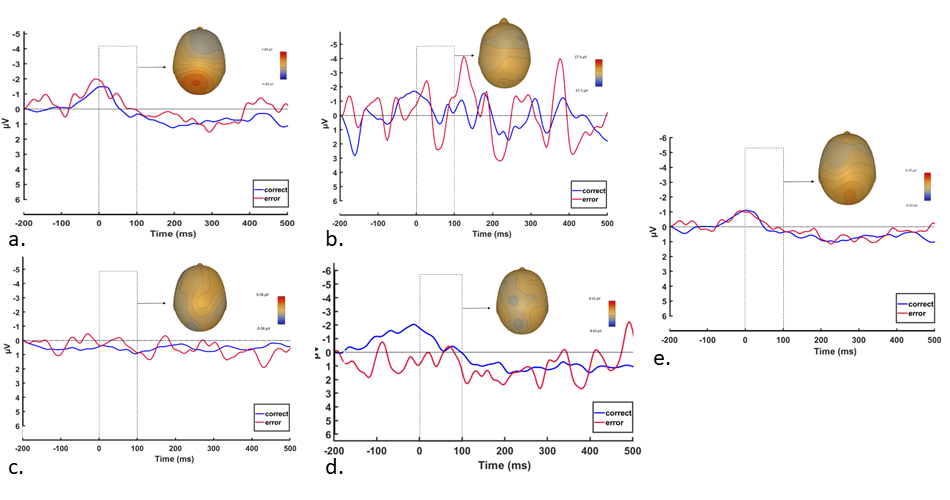
\includegraphics[width=\textwidth]{articles/empirical/traxler/figure3.png}
    \caption{Response-locked grand average waveforms for ERN and CRN at Cz with topography, averaged for (a) the \emph{100\% coactivation task} (N = 5); (b) the \emph{50\% coactivation task} (N = 2); (c) the \emph{Sequence task} (N = 1); (d) the \emph{Different intensities task}
(N = 1); and (e) averaged across the four task versions (N = 9).}
    \label{fig:3}
\end{figure*}


\phantomsection 
\addcontentsline{toc}{section}{Discussion}
\section*{Discussion} 
\gotoreview
\label{sec:discussion}

\noindent Here we describe the piloting of a novel paradigm based on the integration of two experimental tasks stemming from different fields of psychology. Our aim was to develop an instrument suited to measure both the neural activity during error commission that is followed by a negative consequence, namely pain, and the avoidance tendencies in direct response to these pain-evoking errors. As described above, this task is required to evoke an ERN and allow for its reliable measurement ($\mathrm{\ge}$ 6 errors), evoke conscious errors of inhibition in order to allow participants to avoid the painful stimulation, and create sufficient variability in avoidance behavior ($\mathrm{\ge}$ potential avoidance trials, i.e., error trials, and adequate balance between costs and benefits of avoiding vs. not avoiding). Altogether, six different task versions were put to test, which are discussed in the following.

The first task using only \textit{two tactors} proved to be too easy, based on the low number of mistakes made and the reported feedback of the participant. Despite the low perceptual acuity at the lower back, the vibrations were reportedly clearly distinguishable and after a first orientation during the practice phase, the participant had no difficulty completing the task. Consequently, it was decided to add a third vibrotactor to the paradigm to distract from the target stimulation, which resembles the distracting flankers of the Eriksen Flanker task.~

The \textit{Distractor task}, the first version using the third tactor, was programmed to emit vibrations in the rhythm of famous songs which the participant was instructed to identify whilst responding to the left and right vibrations. This task turned out highly demanding, leaving the participant focusing entirely on the discrimination task. Although this version successfully elicited a considerable number of errors, according to the participant the task load interfered with performing the avoidance response, which was perceived as disruptive, such that none of the e-stim were avoided.

In order to decrease the demands of the task, we switched to the \textit{100\% coactivation task}, in which the third tactor coactivated with the target tactor on each trial. On average, participants made a sufficient number of errors for ERN analysis, and allowed for a reasonable variability in avoidance responses. While this version in principle did meet the pre-specified requirements, we decided to further modify this task in an attempt to ensure that the majority of participants would commit sufficient errors.~

First, the \textit{vibration intensity} of the third tactor was slightly increased with the aim to better mask the vibrations of the other tactors. This led to the participant being unsure about their performance and thus unable to perform the avoidance behavior. Second, after setting the vibration intensity of the third tactor back to its original level, we changed the \textit{coactivation to 50\%} of the trials with the goal of increasing unpredictability. Contrary to our expectations, participants experienced this version as easier than the 100\% coactivation version and made fewer mistakes.

Lastly, in the \textit{Sequence task}, participants were asked to perform a sequence of responses repeating after the vibrotactors. Given the speed of the task, it was hypothesized that participants would be easily led into committing errors of inhibition. This approach was successful for one participant; nevertheless, it appeared that the activation of both target tactors within one trial helped the other participant to orient towards the stimulation locations, causing a large difference in the amount of error commissions.~

Overall, the tasks succeeded in eliciting an ERN at fronto-central sites when participants committed errors, which resembled the typical ERN as observed in more classic tasks such as the Eriksen Flanker task (Imburgio et al., 2020). It is noteworthy that the ERNs produced by the different task versions were slightly less pronounced and some peaked earlier than typically found with the Flanker task (Hajcak \& Foti, 2008). Moreover, whereas commonly the reaction times for error trials are found to be shorter than those for correct trials (Aarts \& Pourtois, 2010; Imburgio et al., 2020), the opposite pattern was found in all of the piloted versions of this paradigm. However, a study that compared the ERN elicited by errors on the visual Flanker task with an interoceptive discrimination task using respiratory stimuli reported that the interoceptive ERN (intERN) did peak significantly earlier than the exteroceptive ERN (Tan et al., 2019). The authors argue that interoceptive stimuli might be more relevant for survival, making the detection of interoceptive errors a priority. It is conceivable that somatosensory errors indicating proximal threat, too, carry this relevance and thus evoke a similarly early-peaking ERN, allowing for fast adaptation of behavior. In addition, deviations of the present ERN waveforms from those observed in previous studies are most likely also related to the small number of averaged trials and/or participants (Luck \& Kappenman, 2011).

In conclusion, out of the six versions the \textit{100\% coactivation} task proved the most reliable and useful for investigating whether individuals with larger ERN amplitudes are more prone to engage in pain-related avoidance behavior. Nevertheless, this task does have several limitations: \textit{Firstly}, error commissions may remain low for a fair number of participants, so that it can be expected that a study employing this paradigm will lose many participants on the exclusion criterion of twenty errors that are needed to obtain a useful assessment of avoidance behavior. \textit{Secondly}, the operationalization of avoidance behavior as a single button press may be considered simplistic. Persons with chronic pain tend to engage in a broad variety of, frequently subtle, alternative behaviors and withdrawal from activities that are thought to evoke or worsen their pain. Capturing this complexity in an experimental paradigm is highly challenging, and even though better approximations than button presses do exist (e.g., Meulders et al., 2016), the constraints of the Flanker task, a speeded reaction time task, do not allow for longer, more complex avoidance behaviors in between trials. \textit{Thirdly}, in line with this limitation, engaging in avoidance behavior bears no cost in this paradigm which causes a discrepancy with real-life avoidance where patients are faced with considerable costs to their social life, physical functioning and personal well-being (Martinez-Calderon et al., 2019; Prkachin et al., 2007; Vlaeyen \& Linton, 2012; Wiech \& Tracey, 2013). Yet, when exploring options to add an avoidance cost, in the trade-off between these costs on the one hand and receiving a painful stimulus on the other, participants clearly favored the latter: Participants were instructed that engaging in avoidance behavior would have the consequence of trials being added at the end of the task. As this did not only prolong the duration of the experiment but also further increased the likelihood of error commission, participants appeared to prefer enduring the e-stim. In an attempt to balance the trade-off and increase the cost of not avoiding, the painful stimulation was made more threatening by stating that a "stimulus with a slightly higher intensity than the one previously calibrated" could be delivered occasionally. Surprisingly, this change, too, did not increase the number of avoidance responses. Adjusting the painful stimulus in length or quality was not feasible given the timing of the trial flow. Based on the low levels of avoidance behavior throughout the pilots, possibly due to the cognitive demand of switching from the discrimination task to avoiding the painful stimulus, a surge in avoidance responses is not expected. Moreover, low-cost clinical avoidance, such as constantly carrying pain medication, is common and may be problematic as it impedes treatment and maintains fear (van Vliet et al., 2018; Vervliet \& Indekeu, 2015; Volders et al., 2012). Hence, studying these low-cost avoidance behaviors is clinically relevant, and it was decided not to integrate any further avoidance costs.

Apart from these task-specific limitations, two limitations of the piloting process need to be mentioned: On the one hand, the small and unequal sample sizes for the different task versions do not allow extensive statistical comparisons. On the other hand, some changes to the paradigm were made simultaneously, making it impossible to disentangle the individual effects. The decisions to further modify the paradigm were made as soon as clear converging evidence was obtained from behavioral performance and self-report that a given version was either too easy or too complex, often after just one or two pilots, in order to save time and participants. While this allowed us to try out various ideas and establish a functional paradigm within a few weeks' time, the paradigm clearly requires validation in future studies.

Altogether, developing this experimental task based on the integration of two well-established paradigms was demanding, despite the relative simplicity of the original paradigms. Although the Flanker and the avoidance task seemed compatible on account of their short response intervals and general set-up, many problems arose with regard to timing, task difficulty and interference of responses, and possible solutions often caused unexpected side-effects to participants' behavior. Therefore, a thorough and extensive piloting was pivotal in identifying various pitfalls and re-adjusting the task. In the following section, we have compiled a list of recommendations for those planning to create a novel experimental paradigm.


\phantomsection 
\addcontentsline{toc}{section}{Tutorial}
\section*{Tutorial} 
\gotoreview
\label{sec:tutorial}

\noindent 
This pilot study was an interesting, highly instructive journey. Based on this experience, we propose five key elements to consider when developing a new experimental paradigm or merging existing ones.

\begin{enumerate}
\item  Clarity: Prior to designing the experimental paradigm, it is advised to clearly define the requirements the paradigm ought to meet. One should consider any known necessities or restrictions inherent to the subject or to the original tasks. Relevant questions in this step are ``What is the ultimate goal of this paradigm?'', ``How do I operationalize the independent and outcome variables?'', ``What does this operationalization require in terms of equipment and measurement?'' and ``Which other variables need to be controlled for?''.

\item  Thoroughness: Developing a novel experimental paradigm, even if it seems straightforward, requires thorough piloting, perhaps of several different approaches, and is often a process of trial and error. Keeping a detailed record of decisions, adjustments and their motivation as well as problems encountered, is crucial to understand what works and what does not, and to compare different versions of a paradigm. Furthermore, it is advised to check all relevant data as seemingly small adjustments of a task may have major effects on participants' perception and behavior.

\item  Curiosity: When it becomes clear what does not work, the follow-up question should be ``Why does it not work?''. Exploring the problem more closely may lead to its solution and an improvement of the paradigm. Hence, it may prove useful to include additional measures during the pilots: for example, in studies with human subjects the researchers may choose to use a post-experimental questionnaire that addresses participants' experience of the task as a whole and of any manipulations, as well as their understanding of instructions and materials. Preparing these questions ahead of the pilots, asking them systematically and adjusting them based on new insights may provide valuable information from a different perspective.

\item  Creativity \& Collaboration: Sometimes, a problem in the paradigm cannot be easily fixed. Researchers are well-advised to seek inspiration in directly and indirectly related literature, to reach out to or work together with researchers experienced in the respective domains, and to test the paradigm both on themselves and colleagues to broaden their perspective.

\item  Perseverance: Developing new paradigms or integrating existing ones takes time. We strongly advise to allow for sufficient time to run several pilots, especially if a version of the paradigm seemingly meets all requirements. A well-tested paradigm will minimize the risks during data collection.
\end{enumerate}


\phantomsection 
\addcontentsline{toc}{section}{Conclusion}
\section*{Conclusion} 
\gotoreview
\label{sec:conclusion}

\noindent Developing a novel experimental paradigm is a challenging endeavor that necessitates good preparation and thorough evaluation through extensive piloting. We advise to clearly specify the task requirements in advance, record all problems and applied solutions, and remain open-minded for unconventional approaches and inspirations from various sources.

%\phantomsection \addcontentsline{toc}{section}{References}

\newpage

\phantomsection
\addcontentsline{toc}{section}{Peer Reviews}
\section*{Peer Reviews}
\label{sec:reviews}

\noindent % Paracol is required to make the pagebreak work properly
\begin{paracol}{2}
\begin{reviewend}{Ilona Domen}
    \begin{enumerate}[label=\textbf{\arabic*}), start=0]
    \item \textbf{General comments}
        \begin{enumerate}
            \item The manuscript describes the development and pilot testing of a new paradigm/task, to measure the ERN and avoidance behavior (related to pain) simultaneously. In general I think the manuscript was well written, understandable, and I applaud their efforts in making and recording a new paradigm (and reporting on the whole process) as well as producing a tutorial section. The manuscript did raise quite a few questions for me, and I do have some comments (and concerns) which I describe below. 
            \item I assume the references guidelines follow the APA 6/7 rules. Regarding this, the manuscript should be checked on APA guidelines (especially results, tables, and references).
        \end{enumerate}

    \item \hyperref[sec:introduction]{Introduction}
        \begin{enumerate}
            \item The introduction misses some important references, such as for ERN literature (Gehring and colleagues). Few sources (and few different authors) are mentioned in the introduction in general, which should be extended. More research has been done on these topics (ERN, avoidance behavior) and more than one research should be referenced. The number of errors needed for an ERN only states one source and the number of opportunities to detect avoidance behavior (20) states no source.
            \item Might be due to word count restrictions, but the introduction is rather short and it therefore feels like it does not explain the full circle of reasoning (pain -- avoidance -- more pain and fear; link ERN, why this component. Feedback is also stated, so why not the FRN; neural underpinnings, but there is no mention of fMRI research?). Also the specific need of a task that combines ERN and avoidance behavior (because goal use it in future research / no task exists / separate tasks will not provide the information needed) could be more pronounced (i.e., need/purpose research?). Also, some choices lack motivation/reasoning, such as: `In addition, the task ought to evoke inhibition errors rather than mistakes due to lack of skill or knowledge' (this also occurs in the method/results sections, for example for the exclusion criteria (sources?)).
            \item I feel like (part of) the goal of the research is clear, however, it is not clear to me whether this task is meant to be used in future research (of the researchers themselves or others). The conclusion of this manuscript leaves me wondering whether the task will actually be used or not. The manuscript focuses on three things in my opinion: pilot testing a new task, describing and trying to explain (the not useable) data, and a tutorial. Maybe less focus on analyzing/interpreting data leaves more room for a more detailed tutorial (choices made and why, what went wrong how to fix it, roadmap for others). 
            \item The introduction and discussion mention a criterion of ``at least 20'' [\hyperref[sec:introduction]{introduction}] errors ``needed to obtain a useful assessment of avoidance behaviour'' [\hyperref[sec:discussion]{discussion}]. How was this criterion decided upon? Contrary to the criterion for the minimum number of ERNs, no reference is provided. New tasks are often introduced as aiming at raising the number of errors, but the `why' behind this aim is only elaborated upon in the first paragraph of the discussion, which is too late (and, for me personally, was hard to understand).
        \end{enumerate}

    \item \hyperref[sec:methods]{Methods}
        \begin{enumerate}
            \item I miss the justification of several choices made in the method and data analysis sections (e.g., rationale for bandpass filters, epoch length, 250hz for data acquisition [normally at least 500hz]), using only one electrode (Fcz). 
            \item There are no scales mentioned in the measures section (open questions?).
            \item Some small questions regarding the general procedure: number of trials, number of blocks, what if participants did not press any button to indicate the location of the vibration, controlled for handedness of the participant (normal for EEG), also index finger might be more used for button presses than other fingers. And regarding the different task versions: why did participants have to guess the song, and why was it not good they were aware of the song; how was it known that participants were less aware of the errors they made in the different intensities task.
            \item This manuscript would benefit greatly from a more structured overview of all tasks (\textit{N}, trials, blocks, distractor yes/no, places of vibrations, song yes/no, changes relative to other task versions, choices made and why etcetera) in general, and very early in the method section. This would be a very strong point in this manuscript and would benefit other researchers very much (I made new paradigms myself and would have benefitted from it greatly I think). At this point while reading the manuscript it is a bit chaotic and hard to follow (concepts such as distractor tactor are mentioned early without the reader knowing that it is used or its role, and task names are also non-explaining). The task versions are then explained one by one, with no clear overview of what is different than the one before (and if the evaluation is more positive or negative, and why some adjustments are made). It is one of the strengths of the manuscript in my opinion, and a very structured and detailed overview would be very informative (also since the goal of the manuscript is also a tutorial section).
            \item The low number of participants is understandable given the experiments are time-consuming (I made new paradigms myself). However, one participant per paradigm might be insufficient (especially since error commission differs greatly between participants, and you need a reliable measure, and as it seems in the manuscript, avoidance behavior as well). Also, some paradigms had more participants (so not equal across paradigms), but almost all participants received the penalty for avoiding errors (extension of trials) which distorts the actual measure of avoidance behavior. It also seems that the stimulus was not painful (enough) since participants did not avoid (but it could have another reason). Also, the number of blocks differed per paradigm (and participant), and changes to the paradigms were not tested one by one, but often several changes together. Subtle changes can even make large differences (neural). This pilot testing (with the goal to make a usable task for research) could benefit greatly from consistency. Is there a possibility to collect more data (even on colleagues maybe)?
        \end{enumerate}

    \item \hyperref[sec:results]{Results}
        \begin{enumerate}
            \item I am not sure whether this manuscript should focus on data analysis (too small samples). Could use more space for task overview and tutorial for example
            \item Results should follow APA guidelines?
            \item Why were no EEG data collected for the distractor task and the two tactor task?
            \item `This might indicate that participants are unaware of having committed an error and thus are unable to avoid'. Or they did not want to avoid because of penalties/higher intensity pain stimuli?
            \item Most errors occurred in the first two blocks of all task versions, but if the first 2 blocks generally evoke the most errors, then for participants with only 1 or 2 blocks, the data are less insightful?
            \item The $\Delta$ ERN values need some direction/reference values (what is small/large/preferred/good{\dots}).
            \item Figure 3. Response-locked grand average waveforms for ERN and CRN at Cz with topography. But Fcz was measured for the ERN?
        \end{enumerate}
        
    \item \hyperref[sec:discussion]{Discussion}
        \begin{enumerate}
            \item Are there other tasks normally used to measure ERN or avoidance behavior that might work better together (when they are integrated)?
            \item Conclusions after the task version discussions are missing (for example, two tactor task was inable to detect the ERN due to lack of error commissions, but avoidance behavior was measurable? Therefore we decided to change{\dots}). What is the best version of the task, the 100\% co-activation task? But is it ready/useable for research? What needs to be adjusted? Would you use it for your own research, or recommended it to others (or why is it not tested further)? As long as choices are explained, it is more acceptable.
            \item Why were no EEG data collected for the distractor task and the two tactor task?
            \item I miss the role of the penalties in the discussion of the task versions.
            \item I miss references in the discussion section.
            \item `It is noteworthy that the ERNs produced by the different task versions were slightly less pronounced and some peaked earlier than typically found with the Flanker task (Hajcak \& Foti, 2008)'. I miss the mean ms of the peaks. Could it be less pronounced because participants were unaware of the errors they made? Or why do you think this is? Results are also hard to interpret due to small sample size, few trials and blocks? In my opinion the results/discussion should not focus on interpreting EEG data?
            \item In the discussion section it is mentioned that an option to add avoidance costs (resembling real-life avoidance costs in pain patients) was examined. Then it is better understood why a penalty was added which seemed to undermine the measure of avoidance behavior. Mention this earlier on?
            \item I am curious about these options: `better approximations than button presses do exist'.
            \item `Although the Flanker and the avoidance task seemed compatible on account of their short response intervals and general set-up, many problems arose with regard to timing, task difficulty and interference of responses, and possible solutions often caused unexpected side-effects to participants' behavior. Therefore, a thorough and extensive piloting was pivotal in identifying various pitfalls and re-adjusting the task. In the following section, we have compiled a list of recommendations for those planning to create a novel experimental paradigm'. I completely agree with the extensive and thorough testing, although despite much work, time, and attention was spend on this research, I feel like this did not completely happen. Also especially all the problems could be more extensively documented?
        \end{enumerate}
        
        \item \hyperref[sec:tutorial]{Tutorial}
            \begin{itemize}
                \item When I saw that the manuscript included a tutorial section, I was really enthusiastic about this fact. I believe researchers should share their experiences (good and bad) in performing research, running lab experiments, and especially trying to make a new paradigm more often. I am glad this journal provides an opportunity to do so. It saves other researchers a lot of time (what does not work, what does work, learning from each other's experiences). However, this tutorial provides good insights, but remains on the surface and could go more in depth (for example on problems, solutions, choices made).
            \end{itemize}
            
        \item \hyperref[sec:conclusion]{Conclusion}
            \begin{itemize}
                \item All in all I think this manuscript could be more insightful than it already is, with small (and big) adjustments. I made new paradigms myself, and I think I would have been very much helped with experiences from other researchers, so not everyone has to invent the wheel again. This manuscript could be a nice step towards more open research practices, and sharing research experiences. 
                \item Therefore, I would recommend a \textbf{Revise and Resubmit} of the manuscript.
            \end{itemize}
    \end{enumerate}
%    \tcbsubtitle{Editor}
%    \begin{itemize}
%    \item 
%    \end{itemize}
\end{reviewend}

\begin{reviewend}{De Groot}
    \begin{enumerate}[label=\textbf{\arabic*}), start=0]
    \item \textbf{General comments}
        \begin{itemize}
            \item The present manuscript describes the development and piloting of an experimental task that simultaneously measures Event-Related Negativity (ERN) potentials during error commission, and the avoidance behaviour in response to these pain-evoking errors. This new task integrates two existing tasks: a tactile version of the Eriksen Flanker task and a fear-avoidance paradigm. The new task was piloted using a sample of n = 12 participants, and was continuously adjusted based on the pilot results, resulting in a total of six examined task versions. The focus of the present paper is the development and design of these different task versions, and how such a process ensues (including experience-based tips in the tutorial). The long-term goal of the project is to apply the paradigm to the aetiology of chronic pain, hypothesising that individual differences in ERN amplitude are related to differences in pain avoidance behaviour, with persons with larger ERNs being at risk of developing chronic pain.
            \item The manuscript is characterised by several strengths. In particular, it is very well written. The text has an appropriate level of depth, and has a good flow. Arguments are presented in a concise and clear way, but are still approached from different perspectives. Finally, the paper's main focus is innovative and fits well with the aims of JOTE (as described in its manifesto).
        \end{itemize}
    
    \item \hyperref[sec:introduction]{Introduction}
        \begin{itemize}
            \item The introduction states that ``One of the most prevalent explanations for the transition from a common acute pain episode to chronic disabling pain is the fear-avoidance model'', which ``posits that pain-related avoidance behaviour, often fuelled by catastrophic (mis)interpretations of pain, contributes to individuals entering into a downward spiral of fear, avoidance, inactivity, disability and negative affect'' [...]. While this explanation is indeed prevalent, it is confined to cognitive and behavioural mechanisms, thereby leaving out biological explanations. I feel like it would be fair to readers to provide a broader perspective and also discuss an equally prevalent explanation for chronic pain that focuses on the neural level: the sensitisation model. (I understand that this is not the model the present paper builds on, so a brief description would suffice.) The sensitisation model posits that after an acute pain episode the body hypersensitises the (local) nerves in an attempt to protect the damaged tissue and let it heal. This facilitates triggering pain, reminding the organism to be careful with the damaged tissue. In some cases, hypersensitivity remains, and can spread to other tissues as well. It then becomes a spiral in which the hypersensitivity triggers pain, and the pain in turn hypersensitises the nerves, and so on. See for example \href{https://www.sciencedirect.com/science/article/pii/S1524904210000329}{https://www.sciencedirect.com/science/article/pii/S1524904210000329} and \href{https://www.ncbi.nlm.nih.gov/pmc/articles/PMC1820749/}{https://www.ncbi.nlm.nih.gov/pmc/articles/PMC1820749/}.
            \item The introduction stresses the importance of the ERN for error processing, but what about the Pe (peaking at 200-400 ms, also originating from the ACC)? For readers (somewhat) familiar with error processing literature, the choice of the ERN over the Pe could be confusing, and I would advise the authors to briefly explain their choice.
        \end{itemize}

    \item \hyperref[sec:methods]{Methods}
        \begin{enumerate}
            \item In its present form, I observe one major concern with the manuscript: the sample size used for the piloting. Merely n = 12 participants (n = 10 for the EEG) performed one of six task versions, with three of the piloted tasks having a sample size of just 1, and two having a sample size of 2. Hence, most decisions (like whether a task version satisfied the pre-defined requirements) were made based on only a few datapoints. For example, the two tactor task was deemed too easy based on the data (feedback and number of errors) of just participant, who could easily have been an outlier. In general, the extremely small samples make that data can easily be coincidental rather than structural, even if the results (from that one person) seem very apparent. Related to this, the statistical analysis section (correctly) states that the study has insufficient power for inferential statistics, but I wonder whether non-parametric tests and comparing descriptive statistics acceptable here. The task is newly developed and its score distributions are (yet) unknown. Hence, comparing task versions using only one or two scores per version (which can originate from anywhere on the distribution) is relatively prone to chance. The large number of trials participants obviously compensates for this a bit, but far too little. As a result, I think not much can actually be concluded from the current piloting data (which the authors agree on with regard to the hypothesised link between the ERN and avoidance). As for the reason such a small sample was used, the authors mention saving `time and participants' [\hyperref[sec:discussion]{discussion}], to which I am truly sympathetic, but I do think the extra cost of more participants would have been worth it considering the likely gains of a larger sample. I would like to hear the authors' take on all of this, and would like to suggest three ways to mitigate these issues in the present paper and/or in the future:  
            \begin{itemize}
                \item To me, this issue is a methodological error, which JOTE aims to publish to support learning in the scientific community. However, to educate others, I think the issue should be given more thought in the text, possibly in the limitation section and/or the tutorial section if the authors have any concrete recommendations for mitigating it.
                \item Could it be useful to set a predefined number of participants to be tested for every new task version (like n = 10)? This is still underpowered but would make the decision to modify and retest the paradigm less arbitrary (i.e., less based on what at any moment `seems' right based on the responses of only a few people). It would reduce the risk of decisions being driven by chance findings that look straightforward -- but are not. Such a recommendation could be added to the tutorial if the authors deem it useful as it does reduce some of the flexibility of their current approach). This predefined number could even be included in a preregistration (see more on preregistration below). Alternatively, could doing a power analysis before piloting every new task help? I understand that these changes would increase the costs for this project, but also think that they would reduce the need for and cost of further, more extensive validation.
                \item Like the rest of the manuscript, the results section reads very nicely. One would almost forget that the results hinge on few data. I think it would be fair to readers to integrate Table \ref{tab:manipulations} and \ref{tab:eeg} so that one immediately sees on what sample size a result is based.
            \end{itemize}
        \end{enumerate}
    
    \item \hyperref[sec:participants]{Participants}
        \begin{itemize}
            \item Did participants receive (monetary) compensation for participating? This is not mentioned in the paper, and neither is the origin or recruitment of the participants (they seem a bit old to be regular college students; is it a general population sample?).
        \end{itemize}
        
    \item \hyperref[sec:procedure]{General procedure}
        \begin{itemize}
            \item While the newly developed task is explained in detail, the two tasks it is based on, an Eriksen Flanker task and an avoidance task, are not. For readers unfamiliar with at least one of these base tasks, the lack of a brief, to the point explanation of what they involve makes the concept of the new task difficult to understand in early parts of the paper. Adding this information to the introduction would vastly benefit overall understanding. 
            \item Why did the authors opt for a \textit{tactile} Eriksen Flanker task? Wouldn't a regular (visual) Flanker task that triggers painful stimulation when making a mistake also be able to measure an ERN and avoidance behaviour. 
            \item Compared to its predecessor, the 100\% coactivation task 1) adds a distractor tactor; 2) tells participants that extra trials are added for avoiding pain; and 3) threatens them with triggers that are more painful. Not all participants were presented with all three changes, but Table 1 and 2 only report on the overall results for this task version. It would be helpful to see exactly what number of participants performed which subversion (Table 1), and what the results for those subgroups were (Table 2).
            \item For some task versions it is unclear what the `base settings' are. For example, for the 50\% coactivation task I was not sure whether the different intensities were still in place, hence if the 50\% coactivation scheme was superimposed on the previous scheme or \textit{black} it. Again, extending the information in Table 1 would help here. Note: I often thought versions were better explained in the discussion than the procedure section.
        \end{itemize}
    
    \item \hyperref[sec:sequence]{Sequence task}
        \begin{itemize}
            \item The reasoning behind the development of the sequence task was unclear to me. It doesn't seem to logically follow from the previous task versions.
        \end{itemize}
        
    \item \hyperref[sec:results]{Results}
        \begin{enumerate}
            \item Like the rest of the manuscript, the results section reads very nicely. One would almost forget that the results hinge on few data. I think it would be fair to readers to integrate Table \ref{tab:manipulations} and \ref{tab:eeg} so that one immediately sees on what sample size a result is based.
        \end{enumerate}
        
    \item \hyperref[sec:taskperformance]{Task performance}
        \begin{itemize}
            \item I observed three issues in Figure 3:
            \begin{enumerate}
                \item The topography legend is missing.
                \item The windows marked in the Figure do not match the actual analysis window (which is 0-100 ms for all ERNs and CRNs). Possibly partly because of this difference, the ${\Delta}$ERN values in Table 2 seem different from the average difference between the ERN and CRN in Figure 3, which is also confusing.
                \item The Figure portrays measurements at Cz, whereas the analysis is based around FCz. As FCz is a more logical site for examining the ERN, any effect would be more pronounced there. This is again confusing and could explain the apparent discrepancy between what we see in Figure 3 and what we read in Table 2.
            \end{enumerate}
        \end{itemize}

    \item \hyperref[sec:discussion]{Discussion}
        \begin{itemize}
            \item The discussion states that ``many problems arose with regard to timing, task difficulty and interference of responses, and possible solutions often caused unexpected side-effects to participants' behaviour''. Am I correct that these issues are not further elaborated on in the paper? Would this fit in the discussion or tutorial?
        \end{itemize}
        
    \item \hyperref[sec:tutorial]{Tutorial}
        \begin{itemize}
            \item I would like to share several suggestions with regard to the tutorial:
            \begin{enumerate}
                \item I fully agree with point 1, but would like to suggest an addition where one preregisters the requirements that a to-be-developed paradigm should meet. This would, among others, introduce more accountability into the process.
                \item The same is true for point 2: the \href{https://osf.io/}{OSF} platform could for example host a ``detailed record of decisions, adjustments and their motivation'' [...]. Second, I would advise to give an example from the present project on ``it is advised to check all relevant data as seemingly small adjustments of a task may have major effects on participants' perception and behaviour'' [...] to make it less generic or more informative.
                \item The follow-up questions discussed under point 3 are again suitable for a platform such as OSF. This may aid replication and extension attempts.
                \item Point 4 would also benefit from an open-source repository. In addition, collaboration (via a repository) could take place where different labs run new task versions alongside each other for more participants and statistical power.
                \item For point 5, I would extend ``to allow for sufficient time to run several pilots'' [...] to `and sufficient `participants'.
            \end{enumerate}
        \end{itemize}
    \end{enumerate}
%    \tcbsubtitle{Editor}
%    \begin{itemize}
%    \item 
%    \end{itemize}
\end{reviewend}
\end{paracol}


%%% Citations
% Citations are handled by .bib files, which can easily be generated by Zotero, EndRote, Refwords, Mendeley etc. 

%%% Bibliography
% This just outputs all the references regardless of whether they're actually added in the text or not
%\nocite{*}

% This sets the indent of the references to be nice, should be in the .cls
%\setlength{\bibhang}{\parindent}

%\phantomsection \addcontentsline{toc}{section}{References} 
% Prints the bibliography, duh. But also appends the License, Contributions, Acknowledgments, and Conflicts of Interests
%\printbibliography



\end{document}
